\chapter{System architecture}
\label{ch:architecture}

\lhead{Chapter 7. \emph{System architecture}}

TODO.. introduction


\section{Overview}

Our prototype consists of multiple systems that communicate with each other.
The applications are listed below:

\begin{enumerate}
	\item NIPEN/NIP
	\item Front-end
	\item Heart Rate Application
	\item Weight Application
	\item Weight Polling Service
\end{enumerate}

NIPEN or NIP is our server application that consists of an API and a database.
This application is capable of receiving weight and heart rate data and store them in a database.
It is also able to retrieve data from the database and then send it to our front-end, which then visualizes the information sent.
The next three applications are able to send information to NIP.
For instance the heart rate application is capable of measuring a heart rate and then send it to the integration platform.
The two weight applications are able to fetch weight data from HealthVault and send it to NIP.
The main difference between them is that the \textit{Weigh Application} runs on an Android device, while the \textit{Weight Polling Service} runs on a server or a computer.
In figure \ref{figure:abstract-architecture} an abstract architecture is given of how our applications communicate with each other.

We didn't want to make our applications to complicated, duo to time restriction and lack of resources.
Thus we have only concentrated on one user.
What this means is that we have not implemented functionality for storing and displaying data for multiple users.
However our data structures and database tables support more than one user, since they all contain a user ID.
We have however not implemented any logic to handle several users, this was after all not a requirement.
In addition our systems doesn't contain any type of security, i.e. no authentication or data encryption.
The reason for this is that our customer was explicit that security was not a requirement.
Also, our applications are meant to be a prototype to illustrate how a system like this would work.
And hence security is not necessary.

\begin{figure}[h]
\centering
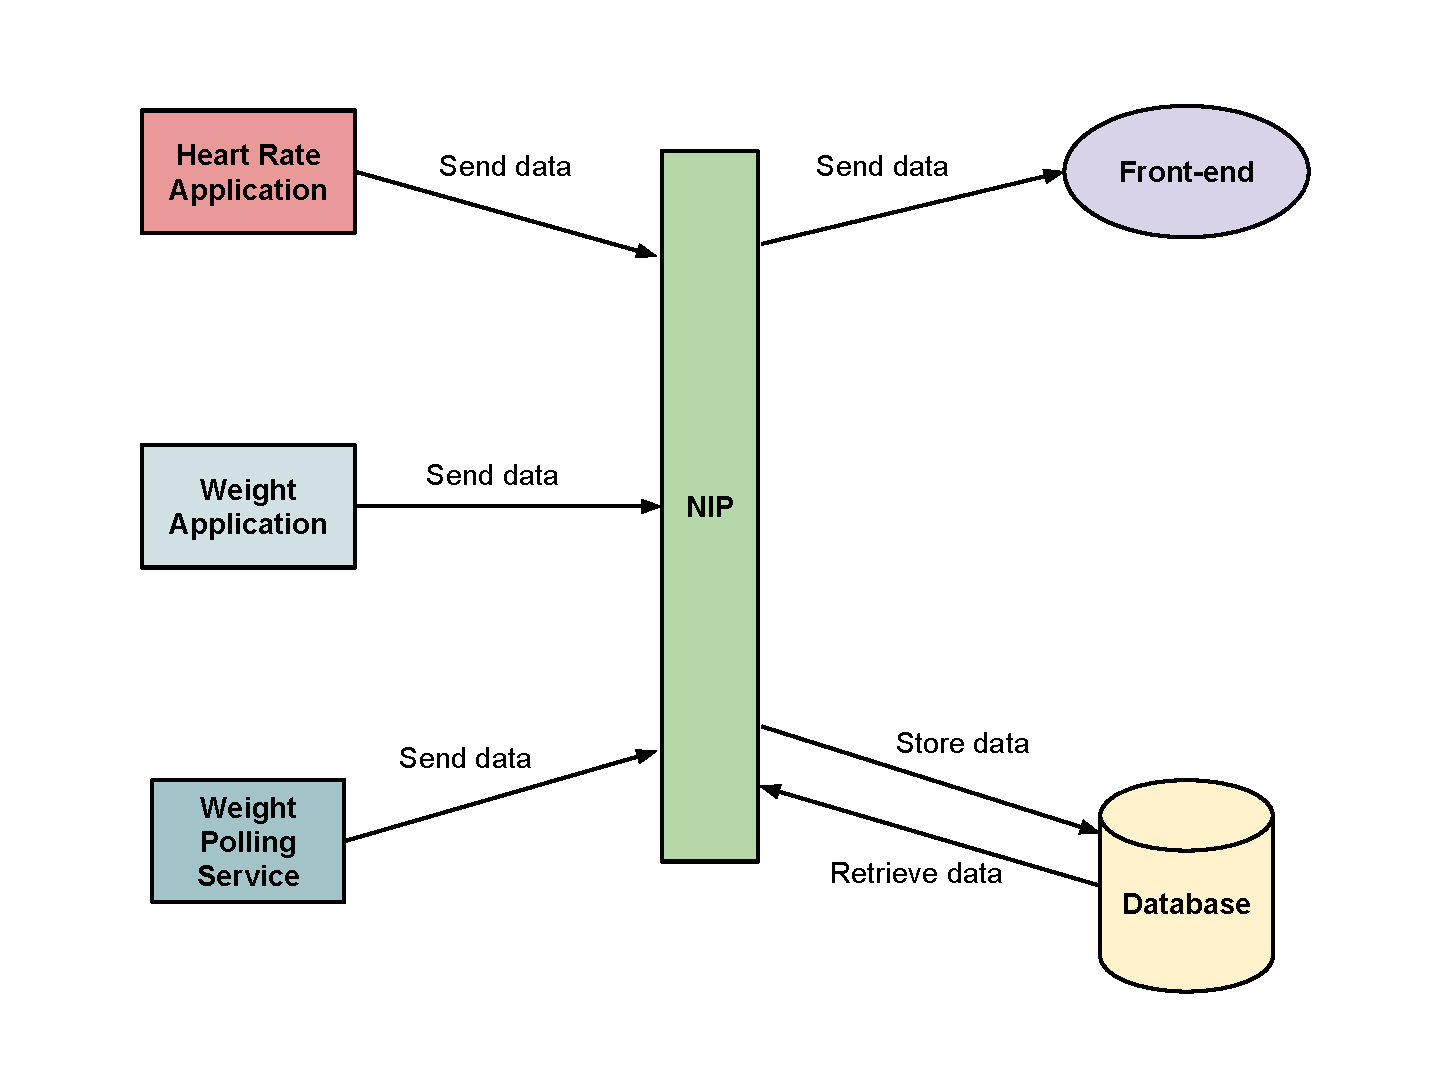
\includegraphics[scale=0.5]{../Figures/abstract-architecture.pdf}
\caption{Abstract architecture}
\label{figure:abstract-architecture}
\end{figure}

\section{NIPEN}

NIPEN is an integration platform for two data types, namely heart rate and weight.
By using the HTTP methods GET and POST it is possible to retrieve and store data into NIP, respectively.
How this works is explained in this subsection.

\textbf{System architecture}

A class diagram containing the most important classes and methods of our system is given in figure \ref{figure:nipen-class-diagram}.

\begin{figure}[h]
\centering
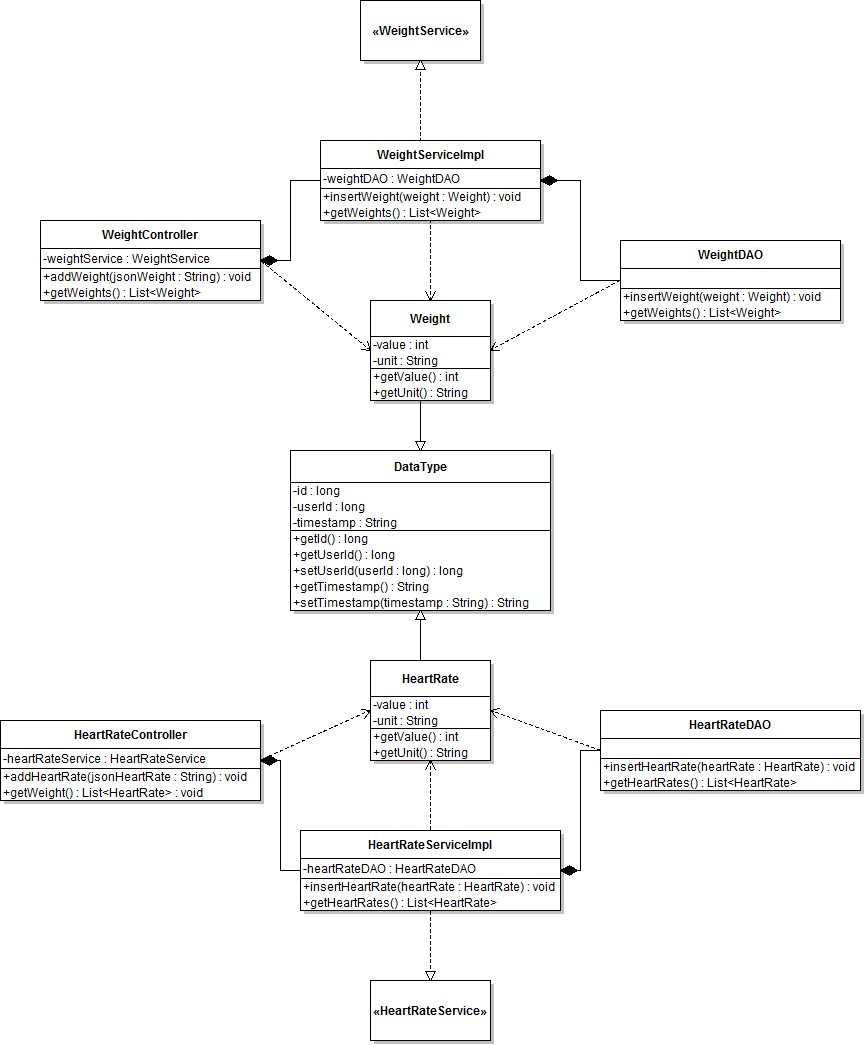
\includegraphics[scale=0.5]{../Figures/NIPEN-class-diagram.png}
\caption{NIPEN class diagram}
\label{figure:nipen-class-diagram}
\end{figure}

We are following MVC (Model-view-controller) architecture pattern. 
What this means is that we have divided our application into three main parts: models, views and controllers.

\begin{itemize}

\item Model: A model is a type of data structure that is used within an application.
In our case the models of our application are: Weight, HeartRate and DataType.
This classes are filled with data from the database and are used when sending data to the front-end.
They are also used to store data into our database.

\item View: A view is something that displays the data from the models to the users.
The front-end is the view in our case.
How the front-end works is described in subsection \ref{subsec:front-end}.

\item Controller: The controller is responsible for updating the models that are going to be used in the view.
In our application the controllers are called when a HTTP GET or HTTP POST request is sent to a specific URL.
The controllers work as an interface that connects the applications we have developed with our back-end.

\end{itemize}

\textbf{Database}

We are using a MySQL database for data storage.
It consists of two tables for each data type, one for heart rate and one for weight.
The heart rate table is shown in figure \ref{figure:heart-rate-database-diagram} and the weight table in figure \ref{figure:weight-database-diagram}. 
As we can see the tables are identical, the only difference is the name.
The reason we didn't merge this tables is to separate the data, and it is also more efficient.
It would require more resources to separate the data if they all were in one table.

\begin{figure}[h]
\centering
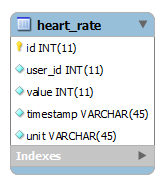
\includegraphics[scale=1.0]{../Figures/heart-rate-database-diagram.png}
\caption{Heart rate database diagram}
\label{figure:heart-rate-database-diagram}
\end{figure}

\begin{figure}[h]
\centering
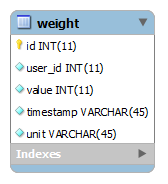
\includegraphics[scale=1.0]{../Figures/weight-database-diagram.png}
\caption{Weight database diagram}
\label{figure:weight-database-diagram}
\end{figure}

We have created separate classes for accessing the database through our server application.
One for heart rate (HeartRateDAO) and one for weight (WeightDAO).
This two classes contain a method for inserting and a method for fetching data from the database.
The data that is fetched from the database is ordered by its time stamp.
In this way the other parts of the system doesn't need to sort the data afterwards.

\textbf{Data format}

We are using JSON strings when transmitting data to and from the server.
The representation of the data is inspired from the Human API.
Both heart rate and weight data is represented with the same attributes.
They contain an ID, user ID, time stamp, value and a unit.
The ID is not needed, when the JSON string is sent, because it is created on the server side.
Below is a representation of a heart rate JSON string that can be used to store heart rate data on the server:

\begin{lstlisting}[language=json]
{
    "userId":1,
    "timestamp":"2013-10-27 14:57:39.0",
    "value":65,
    "unit":"bpm"
}
\end{lstlisting}

A weight measurement can be sent in the same format but should be sent with another unit.
The ID of the data is shown when receiving the data from the server:

\begin{lstlisting}[language=json]
{
    "id":39,
    "userId":1,
    "timestamp":"2013-10-27 14:57:39.0",
    "value":65,
    "unit":"bpm"
}
\end{lstlisting} 

\textbf{API calls}

A RESTful (Representational State Transfer) service is used when communicating with NIPEN.
What this means is that we are using HTTP methods to request and send data.
We have two controllers that handle the API calls, concerning the heart rate and weight data, in our system.
They are called \textit{HeartRateController} and \textit{WeightController}. 
The \textit{HeartRateController} controls retrieval and storage of heart rate, while the \textit{WeightController} handles weight data.
These controllers handle two HTTP methods, POST for pushing data and GET for retrieving data.
When requesting data from our API a HTTP GET request needs to be performed to one of the following URLs:

\begin{itemize}
\item $<$server address$>$/nipen/api/human/heart\_rates
\item $<$server address$>$/nipen/api/human/weights
\end{itemize}

The first URL requests all the heart rates, while the second URL requests all the weights stored in the database.
In figure \ref{figure:retrieve-heart-rates-from-the-database} a sequence diagram is given of how the controller retrieves the data for the user.
The weight controller works the same way.
When the controller receives a HTTP GET request, it contacts a data type service which again contacts a database handler class.
The database handler class returns a list of models which is at last returned to the controller.
The list of models is transformed automatically into JSON string with help of the Spring Framework.
Both controllers will respond with an array of JSON strings representing the respective data.

\begin{figure}[h]
\centering
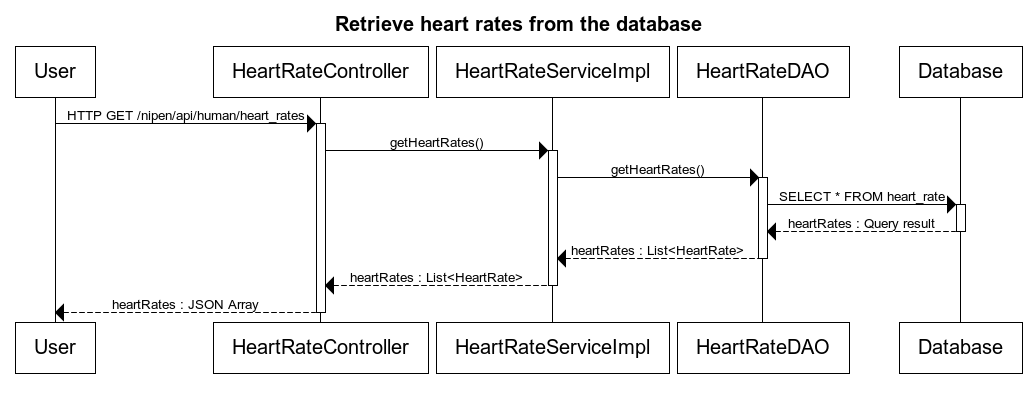
\includegraphics[scale=0.6]{../Figures/retrieve-heart-rates-from-the-database.png}
\caption{Retrieving heart rates from the database}
\label{figure:retrieve-heart-rates-from-the-database}
\end{figure}

To send data to NIPEN one of the following URLs needs to be used with the HTTP POST method:

\begin{itemize}
\item $<$server address$>$/nipen/api/human/heart\_rate
\item $<$server address$>$/nipen/api/human/weight
\end{itemize}

With the POST method a JSON string with the specified data type needs to be sent. 
How the controller handles this message is shown in figure \ref{figure:pushing-weight-into-NIPEN}.
The diagram shows an example of how to push a weight value into NIPEN.
The application works the same way when pushing a heart rate value into the system.
When the application receives the JSON string, it first needs to parse it into its respective model class.
After that it is sent to a service class which then sends it to a database handler class.
This class stores the value into the database.

\begin{figure}[h]
\centering
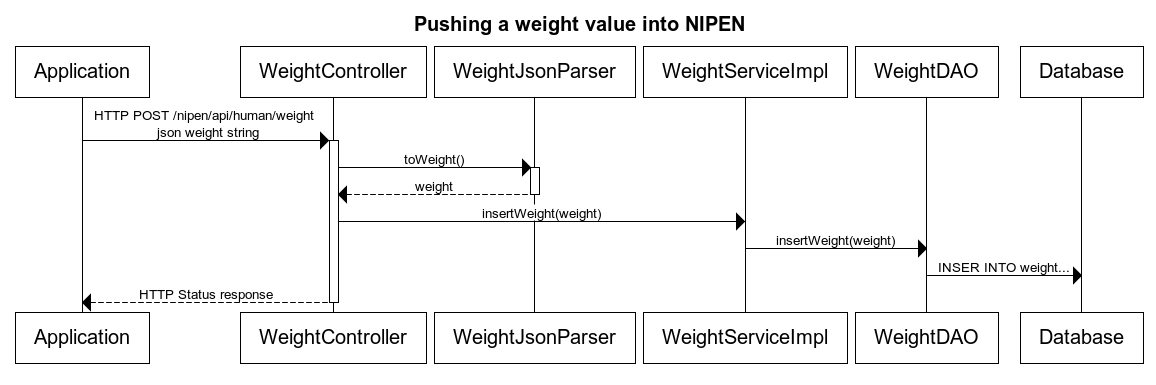
\includegraphics[scale=0.55]{../Figures/pushing-weight-into-NIPEN.png}
\caption{Pushing a weight value into NIPEN}
\label{figure:pushing-weight-into-NIPEN}
\end{figure}

\section{Front-end}
\label{subsec:front-end}

The main functionality of the front-end is to visualize the data stored by the Integration Platform.
This is accomplished by using a regular web-page consisting of HTML, CSS and JavaScript. HTML and CSS is used for structuring and giving a nice design of the web page. With help of JavaScript we are able to make the page dynamic.

\textbf{Design and Visualization}

One of the requirements given by the customer was that the front-end should use helsenorge.no color palette. 
That is the front-end should use the colors shown in figure \ref{figure:helsenorge-color-palette}. 
The front-end should show how helsenorge.no could represent the data from the integration platform. 
Since it would somehow mimic that page, we though that our web page should look similar to helsenorge.no. 
Hence we didn't only use the colors from the given palette, but tried as well to create a similar structure.

\begin{figure}[h]
\centering
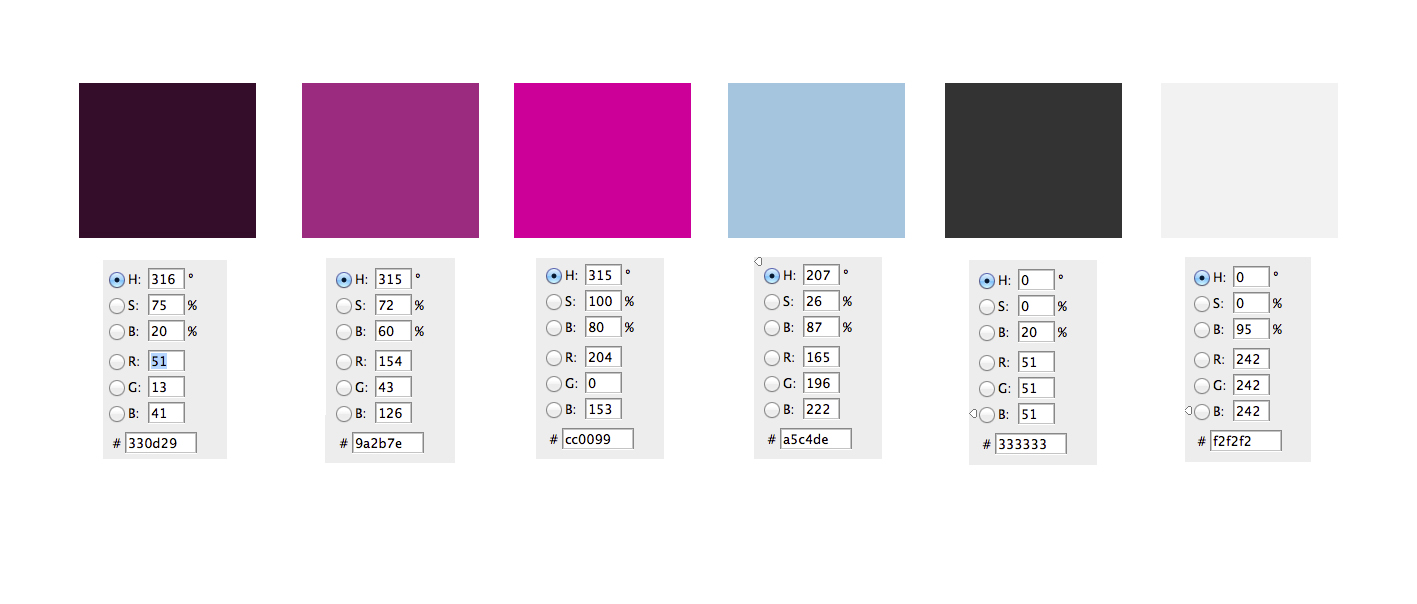
\includegraphics[scale=0.30]{../Figures/helsenorge_pallett.jpg}
\caption{Helsenorge color palette}
\label{figure:helsenorge-color-palette}
\end{figure}

We wanted to keep our front-end simple and user friendly, and since this is only a prototype are we only focusing on one user.
Hence we are only concentrating on how the web page should look like if the user is logged in. 
Therefore we didn't create any authentication page and thus the user doesn't need to log in. 
The front-end simply consists of one HTML file with some CSS and script files.
Twitter Bootstrap was used as a template to get started with the front-end development.
With help of JavaScript combined with jQuery, were we able to have three web pages in one HTML file. 
The main page consists of two graphs, one for heart rate and another one for weight measurements. 
A visualization of the two latest values measured for each data type is also shown on the front page.
Then we have two separate pages for heart rate and for weight.
These pages consists of an enlarged graph of the given data type being viewed.
This is simply accomplished by hiding the elements that are not used on those pages, and scaling the respective graph so it becomes larger.
With help of jQuery it's not a difficult task.
As a bonus jQuery is able to give an animation when hiding, showing and scaling the elements.
This is a nice touch to the web page.

We are using a JavaScript library called Chart.js to display the data received from the back-end. 
With help of this library we are able to display the heart rates and weights as bar charts.
This library also has some animations when the graphs are created.
In our application a restriction is given to only display the 10 last measurements in the graphs.
If we have more than that the time stamp of the measurements becomes hard to read.

\textbf{Retrieving the Data}

TODO

\textbf{Polling}

TODO

\section{Heart rate application}

TODO

\section{Weight application}

TODO

\section{Weight Polling Service}

TODO
